\documentclass[tikz, border=15pt]{standalone}
\usepackage{tikz}
\usetikzlibrary{shapes.geometric, arrows.meta, positioning, shadows, calc, backgrounds, fit}
\usepackage{amsmath, amsfonts}

% 定制现代 AI 调色板
\definecolor{tokenbg}{HTML}{3B82F6}   % 蓝
\definecolor{embedbg}{HTML}{10B981}   % 绿
\definecolor{blockbg}{HTML}{8B5CF6}   % 紫
\definecolor{normbg}{HTML}{F59E0B}    % 橙黄
\definecolor{headbg}{HTML}{EC4899}    % 粉红
\definecolor{logitbg}{HTML}{6366F1}   % 靛蓝
\definecolor{arrowcol}{HTML}{64748B}  % 灰蓝箭头

% 大框所使用的 Slate 板岩灰定义
\definecolor{slate-100}{HTML}{F1F5F9} % 实体背景色
\definecolor{slate-600}{HTML}{475569} % 实线边框色/高级灰文字色
\definecolor{slate-700}{HTML}{334155} % 内部标题背景色

% 分层渲染顺序
\pgfdeclarelayer{modelbg}
\pgfdeclarelayer{stackbottom}
\pgfdeclarelayer{stackmid}
\pgfdeclarelayer{arrows}
\pgfsetlayers{modelbg,stackbottom,stackmid,main,arrows}

\begin{document}
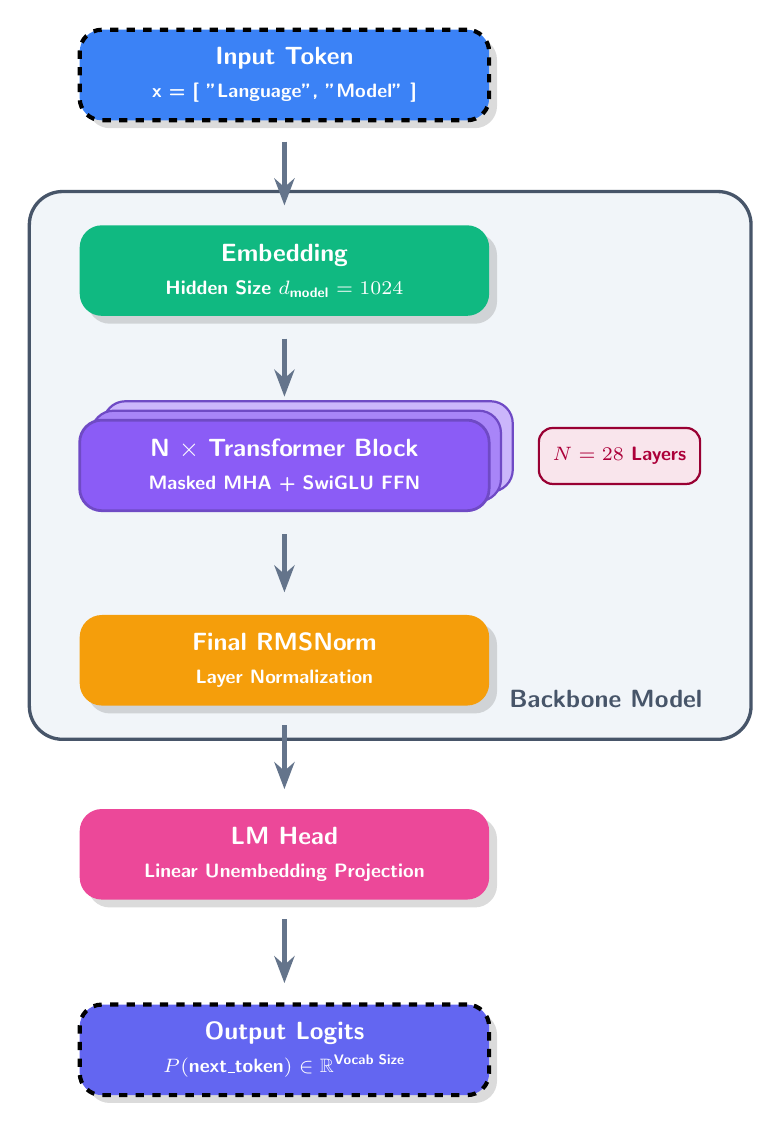
\begin{tikzpicture}[
    node distance=1.3cm and 0cm,
    >=Stealth,
    % 1. 普通模块卡片（带标准阴影）
    box/.style={
        draw=none,
        rounded corners=8pt,
        minimum width=5.2cm,
        minimum height=1.15cm,
        text=white,
        font=\sffamily\bfseries\small,
        align=center,
        drop shadow={shadow xshift=0.10cm, shadow yshift=-0.10cm, fill=black!70, opacity=0.20}
    },
    % 2. Transformer 顶层 Block
    blocktop/.style={
        rounded corners=8pt,
        minimum width=5.2cm,
        minimum height=1.15cm,
        text=white,
        font=\sffamily\bfseries\small,
        align=center,
        draw=blockbg!80!black,
        line width=1.0pt
    },
    % 3. 堆叠背景卡片
    stackbox/.style={
        rounded corners=8pt,
        minimum width=5.2cm,
        minimum height=1.15cm,
        draw=blockbg!80!black,
        line width=0.8pt
    },
    % 4. 数据节点
    databox/.style={
        box,
        draw=black,
        dashed,
        line width=1.5pt
    },
    % 基础箭头样式
    arrow/.style={
        ->,
        line width=1.5pt,
        draw=arrowcol,
        shorten >=7pt,
        shorten <=7pt
    },
    % Block 专属箭头
    blockarrow/.style={
        ->,
        line width=1.5pt,
        draw=arrowcol,
        shorten >=8pt,
        shorten <=8pt
    }
]

    % --- 1. 主节点绘制 ---
    
    % Input Token
    \node[databox, fill=tokenbg] (token) {
        Input Token \\[1pt]
        {\scriptsize x = [ "Language", "Model" ]}
    };
    
    % Embedding
    \node[box, fill=embedbg, below=of token] (embed) {
        Embedding \\[1pt]
        {\scriptsize $\text{Hidden Size } d_{\text{model}} = 1024$}
    };
    
    % N x Transformer Block
    \node[blocktop, fill=blockbg, below=of embed] (block) {
        N $\times$ Transformer Block \\[1pt]
        {\scriptsize Masked MHA + SwiGLU FFN}
    };
    
    % Final RMSNorm
    \node[box, fill=normbg, below=of block] (norm) {
        Final RMSNorm \\[1pt]
        {\scriptsize Layer Normalization}
    };
    
    % LM Head
    \node[box, fill=headbg, below=of norm] (head) {
        LM Head \\[1pt]
        {\scriptsize Linear Unembedding Projection}
    };
    
    % Output Logits (通过 below=of head 精准将底部距离拉紧)
    \node[databox, fill=logitbg, below=of head] (logits) {
        Output Logits \\[1pt]
        {\scriptsize $P(\text{next\_token}) \in \mathbb{R}^{\text{Vocab Size}}$}
    };

    % --- 2. Transformer Block 背景堆叠层 ---
    
    \begin{pgfonlayer}{stackbottom}
        \node[stackbox, fill=blockbg!45] at ($(block) + (0.30cm, 0.24cm)$) {};
    \end{pgfonlayer}
    
    \begin{pgfonlayer}{stackmid}
        \node[stackbox, fill=blockbg!75] at ($(block) + (0.15cm, 0.12cm)$) {};
    \end{pgfonlayer}

    % --- 3. 右侧 Badge 标签 ---
    \node[
        fill=purple!10, 
        draw=purple!80!black, 
        line width=0.8pt,
        rounded corners=5pt, 
        inner xsep=5pt,
        inner ysep=7pt,
        font=\sffamily\scriptsize\bfseries, 
        text=purple!90!black,
        anchor=west
    ] (badge) at ($(block.east) + (0.6cm, 0.12cm)$) {$N = 28$ Layers};

    % --- 4. 连接箭头绘制 ---
    \begin{pgfonlayer}{arrows}
        \draw[arrow] (token) -- (embed); 
        \draw[blockarrow] (embed) -- (block);
        \draw[blockarrow] (block) -- (norm);
        \draw[arrow] (norm) -- (head);
        % 底部收紧后适度缩小缩进，避免线太短
        \draw[arrow] (head) -- (logits);
    \end{pgfonlayer}

    % --- 5. 实线框与右下角框内标题 ---
    \begin{pgfonlayer}{modelbg}
        % 大实线框
        \node[
            draw=slate-600,             % 实线边框
            line width=1.2pt,
            rounded corners=12pt,
            fill=slate-100,             % 实体背景色
            fit=(embed) (norm) (badge),
            inner xsep=18pt,
            inner ysep=12pt             % 上下内边距
        ] (modelbox) {};
        
        % 放置于框内【右下角空白处】的标题卡片
        \node[
            anchor=south east,
            font=\sffamily\bfseries\small,
            text=slate-600,             
            inner xsep=8pt,
            inner ysep=4pt,
            rounded corners=5pt
        ] at ($(modelbox.south east) + (-10pt, 8pt)$) {Backbone Model};
    \end{pgfonlayer}

\end{tikzpicture}
\end{document}